\documentclass[11pt]{article}

\usepackage[margin=1in]{geometry}
\usepackage[T1]{fontenc}
\usepackage[utf8]{inputenc}
\usepackage{lmodern}
\usepackage{microtype}
\usepackage{amsmath,amssymb,mathtools}
\usepackage{booktabs}
\usepackage{tabularx}
\usepackage{array}
\usepackage{xcolor}
\usepackage{enumitem}
\usepackage{tikz}
\usepackage{listings}
\usepackage[numbered,framed]{matlab-prettifier}
\usepackage{hyperref}
\usepackage{cleveref}

\usetikzlibrary{arrows.meta,positioning,calc}

\hypersetup{
  colorlinks=true,
  linkcolor=blue!55!black,
  urlcolor=blue!55!black,
  citecolor=blue!55!black,
  pdftitle={DP-LMI Package User Manual},
  pdfauthor={DP-LMI Package}
}

\lstdefinestyle{dpmatlab}{
  style=Matlab-editor,
  basicstyle=\mlttfamily\small,
  breaklines=true,
  columns=fullflexible,
  keepspaces=true,
  showstringspaces=false,
  frame=single,
  rulecolor=\color{black!20},
  numbers=none
}

\lstdefinestyle{dpoutput}{
  basicstyle=\ttfamily\small,
  breaklines=true,
  columns=fullflexible,
  keepspaces=true,
  frame=single,
  rulecolor=\color{black!20},
  backgroundcolor=\color{black!3},
  numbers=none
}

\newcommand{\pkg}{DP-LMI package}
\newcommand{\matlab}{MATLAB}
\newcommand{\code}[1]{\texttt{#1}}

\title{\pkg\\User Manual}
\author{Version v0.1.0}
\date{July 2026}

\begin{document}

\maketitle

\begin{abstract}
This manual describes the current public behavior of the \pkg.  The present
implementation provides the \code{dpbase} class and shared validation tests for
cell-local Bernstein coefficient storage on tensor grids.  Solver-facing DP-LMI
objects such as \code{dpmat}, \code{dpvar}, and \code{dplmi} are planned package
layers, but they are not yet public APIs in this repository version.
\end{abstract}

\tableofcontents
\newpage

\section{Installation And Verification}

\subsection{Add The Package To The MATLAB Path}

Start \matlab{} in the repository root, or set \code{projectRoot} to the
absolute path of the checked-out repository.  Add the package recursively, then
remove the documentation directory from the executable path.

\begin{lstlisting}[style=dpmatlab]
projectRoot = "path/to/Differential Parameter-Dependent Linear Matrix Inequality";
addpath(genpath(projectRoot));
rmpath(genpath(fullfile(projectRoot, "doc")));
\end{lstlisting}

For local development from the repository root, the shorter form is enough:

\begin{lstlisting}[style=dpmatlab]
addpath(pwd)
\end{lstlisting}

\subsection{Run The Current Test Suite}

The current verification entry point runs the non-SDP tests for \code{+helper}
and \code{@dpbase}.

\begin{lstlisting}[style=dpmatlab]
results = tests.run_all;
table(results)
\end{lstlisting}

Expected result: all currently implemented tests pass.  At the time this manual
was written, the suite contained 30 tests covering helper validation and
\code{dpbase} construction, grid metadata, local storage, label ordering, and
rate-bound validation.

The command above does not verify YALMIP modeling, SDP solver calls, relaxation
lemma assembly, or DP-LMI feasibility workflows because those public layers are
not implemented in this version.

\section{Quick Start}

\code{dpbase} stores one flat Bernstein coefficient cell for each physical cell
of a tensor grid.  The default constructor creates zero numeric coefficient
payloads; it does not sample a function at grid nodes.

\subsection{A Scalar Grid}

\begin{lstlisting}[style=dpmatlab]
obj = dpbase({[0 1 3]}, [2 3], 1);

obj.MatrixSize
obj.Degree
obj.GridInfo.Bounds
obj.npar()
obj.ncell()
obj.ncoeff()
size(obj)
obj.cells()
obj.lbls()
\end{lstlisting}

Expected structural outputs:

\begin{lstlisting}[style=dpoutput]
MatrixSize =
     2     3

Degree =
     1

Bounds =
     0     3

npar()   -> 1
ncell()  -> 2
ncoeff() -> 2
size(obj)-> [2 3]

cells() =
     1
     2

lbls() =
     0
     1
\end{lstlisting}

There are two physical intervals, \([0,1]\) and \([1,3]\).  Because the degree
is one and the grid is one-dimensional, each physical cell stores two local
Bernstein coefficients.

\subsection{Access Local Coefficients}

\begin{lstlisting}[style=dpmatlab]
c1 = obj.coeffs(1);
c2 = obj.coeffs(2);
\end{lstlisting}

Expected result: both \code{c1} and \code{c2} are \code{1x2} cell arrays.  Each
entry is a numeric zero matrix of size \code{2x3}.  The first cell corresponds
to local labels \(0\) and \(1\) on the interval \([0,1]\); the second cell uses
the same local labels on the interval \([1,3]\).

\subsection{A Tensor Grid}

\begin{lstlisting}[style=dpmatlab]
obj = dpbase({[0 1 2], [10 20 30]}, [1 1], 1);

obj.GridInfo.Points
obj.cells()
obj.lbls()
obj.coeffs([2 1])
\end{lstlisting}

Expected structural outputs:

\begin{lstlisting}[style=dpoutput]
GridInfo.Points =
     0    10
     0    20
     0    30
     1    10
     1    20
     1    30
     2    10
     2    20
     2    30

cells() =
     1     1
     1     2
     2     1
     2     2

lbls() =
     0     0
     0     1
     1     0
     1     1
\end{lstlisting}

The first parameter index varies more slowly than the second.  This row order
is used consistently for physical cells and local Bernstein labels.

\section{Bernstein Storage Background}

\subsection{One Cell, Local Coordinates}

On one physical interval \([\rho_0,\rho_1]\), a local coordinate
\(\alpha \in [0,1]\) can represent a degree-\(m\) Bernstein polynomial as
\[
  P(\alpha) = \sum_{i=0}^{m} C_i B_i^m(\alpha),
  \qquad
  B_i^m(\alpha) = \binom{m}{i}\alpha^i(1-\alpha)^{m-i}.
\]
For matrix-valued data, each coefficient \(C_i\) is a matrix with the same
payload size.  \code{dpbase} stores those matrices as a flat cell array.

\begin{center}
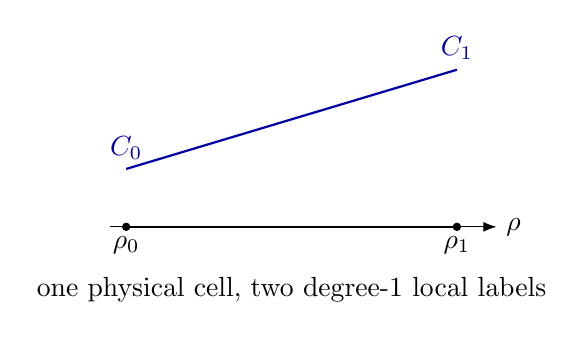
\begin{tikzpicture}[x=4.2cm,y=2.1cm,>=Latex]
  \draw[->] (-0.05,0) -- (1.12,0) node[right] {$\rho$};
  \draw[thick] (0,0) -- (1,0);
  \draw[fill=black] (0,0) circle (1.3pt) node[below] {$\rho_0$};
  \draw[fill=black] (1,0) circle (1.3pt) node[below] {$\rho_1$};
  \draw[blue!65!black,thick] (0,0.35) -- (1,0.95);
  \node[blue!65!black,above] at (0,0.35) {$C_0$};
  \node[blue!65!black,above] at (1,0.95) {$C_1$};
  \node at (0.5,-0.38) {one physical cell, two degree-1 local labels};
\end{tikzpicture}
\end{center}

\subsection{Tensor-Product Labels}

For \(\ell\) parameter dimensions and degree \(m\), each local label is an
\(\ell\)-tuple in \(\{0,\ldots,m\}^{\ell}\).  The number of local coefficients
per physical cell is
\[
  (m+1)^\ell.
\]
For example, \(\ell=2\) and \(m=1\) gives labels
\[
  (0,0),\ (0,1),\ (1,0),\ (1,1),
\]
which is exactly the order returned by \code{obj.lbls()}.

\subsection{Products And Degree Growth}

When two Bernstein polynomials are multiplied on the same physical cell, their
local labels add and the result has the sum of the operand degrees.  The package
contains private implementation utilities for this binomial-scaled convolution
and degree elevation.  These utilities are internal; users should inspect
coefficient ordering through public methods such as \code{lbls},
\code{cells}, \code{ncoeff}, and \code{coeffs}.

\section{\texorpdfstring{\code{dpbase}}{dpbase} Reference}

\subsection{Purpose}

\code{dpbase} is the shared coefficient-backed storage class for gridded
DP-LMI objects.  In this repository version it is also the only implemented
public class.  It stores tensor-grid metadata, matrix payload size, Bernstein
degree, nested physical-cell coefficient data, and rate-dependence metadata.

\subsection{Syntax}

\begin{lstlisting}[style=dpmatlab]
obj = dpbase(gridVectors, matrixSize, degree)
obj = dpbase(gridVectors, matrixSize, degree, localValues)
obj = dpbase(gridVectors, matrixSize, degree, localValues, Name=Value)
\end{lstlisting}

\subsection{Inputs}

\begin{tabularx}{\linewidth}{@{}>{\raggedright\arraybackslash}p{0.25\linewidth}>{\raggedright\arraybackslash}X@{}}
\toprule
Input & Description \\
\midrule
\code{gridVectors} &
Nonempty cell array of grid node vectors.  Each vector must be finite, real,
strictly increasing, numeric, and contain at least two nodes. \\
\code{matrixSize} &
\code{1x2} positive integer vector giving the row and column size of every
coefficient payload. \\
\code{degree} &
Nonnegative integer scalar Bernstein degree. \\
\code{localValues} &
Optional nested cell payload.  If omitted or empty, \code{dpbase} creates zero
numeric coefficient matrices for every local coefficient of every physical
cell. \\
\bottomrule
\end{tabularx}

\subsection{Name-Value Options}

\begin{tabularx}{\linewidth}{@{}>{\raggedright\arraybackslash}p{0.3\linewidth}>{\raggedright\arraybackslash}X@{}}
\toprule
Option & Description \\
\midrule
\code{IsContinuous} &
Logical metadata flag.  \code{dpbase} records the flag but does not enforce
boundary sharing itself.  Future subclasses own continuity construction. \\
\code{ContainsDecision} &
Logical metadata flag for future decision-variable subclasses. \\
\code{HasRateDependence} &
Logical metadata flag.  If true, nonempty \code{RateBounds} must be supplied. \\
\code{RateBounds} &
Empty, or an \(\ell \times 2\) finite real matrix with lower bounds in column
one and upper bounds in column two.  The number of rows must match the number
of parameter dimensions. \\
\code{SourceSummary} &
String metadata describing the coefficient source.  The default is
\code{"coefficient-backed"}. \\
\bottomrule
\end{tabularx}

\subsection{Properties}

All public properties have private set access.  Users can inspect them but
cannot assign to them after construction.

\begin{tabular}{@{}>{\raggedright\arraybackslash}p{0.32\linewidth}@{\hspace{0.02\linewidth}}>{\raggedright\arraybackslash}p{0.58\linewidth}@{}}
\toprule
Property & Meaning \\
\midrule
\code{GridInfo} &
Struct with fields \code{Vectors}, \code{Points}, \code{Bounds}, and
\code{NumNodes}. \\
\code{MatrixSize} & Matrix payload size stored as a \code{1x2} vector. \\
\code{Degree} & Bernstein degree. \\
\code{LocalValues} &
Nested physical-cell storage.  A tensor grid uses nested brace access, for
example \code{LocalValues\{i1\}} followed by \code{\{i2\}} and later dimensions;
each leaf stores a flat coefficient cell. \\
\code{IsContinuous} & Continuity metadata flag. \\
\code{ContainsDecision} & Decision-dependence metadata flag. \\
\code{HasRateDependence} & True when rate metadata or rate-affine payloads are present. \\
\code{RateBounds} & Empty or an \(\ell \times 2\) finite real rate-bound table. \\
\code{SourceSummary} & String metadata for the coefficient source. \\
\bottomrule
\end{tabular}

\subsection{Methods}

\begin{tabularx}{\linewidth}{@{}>{\raggedright\arraybackslash}p{0.31\linewidth}>{\raggedright\arraybackslash}X@{}}
\toprule
Method & Behavior \\
\midrule
\code{size(obj)} &
Return the matrix payload size.  \code{size(obj,dim)} follows ordinary matrix
behavior for dimensions beyond two by returning one. \\
\code{npar(obj)} & Return the number of parameter dimensions. \\
\code{ncell(obj)} & Return the number of physical tensor-grid cells. \\
\code{ncoeff(obj)} & Return the number of local Bernstein coefficients per cell. \\
\code{cells(obj)} & Enumerate physical-cell subscripts in flat row order. \\
\code{lbls(obj)} & Enumerate local Bernstein labels in flat row order. \\
\code{coeffs(obj,cellSubs)} &
Return the flat coefficient cell for one physical cell.  \code{cellSubs} can be
a numeric row vector or a cell array with one physical-cell index per parameter.
\\
\bottomrule
\end{tabularx}

\subsection{Custom Local Values}

For a one-dimensional grid with two physical cells and degree two, each physical
cell must store three local coefficients.

\begin{lstlisting}[style=dpmatlab]
localValues = {{11, 12, 13}, {21, 22, 23}};
obj = dpbase({[0 1 2]}, [1 1], 2, localValues);

obj.coeffs(2)
obj.coeffs({1})
\end{lstlisting}

Expected output:

\begin{lstlisting}[style=dpoutput]
obj.coeffs(2)  -> {21, 22, 23}
obj.coeffs({1})-> {11, 12, 13}
\end{lstlisting}

For a tensor grid, physical cells are nested one parameter dimension at a time.
The storage contract is \code{LocalValues\{i1\}\{i2\}...}, not
\code{LocalValues\{i1,i2,...\}}.

\begin{lstlisting}[style=dpmatlab]
mkCoeff = @(offset) {offset+1, offset+2, offset+3, offset+4};
localValues = {
    {mkCoeff(110), mkCoeff(120)}, ...
    {mkCoeff(210), mkCoeff(220)}
    };

obj = dpbase({[0 1 2], [10 20 30]}, [1 1], 1, localValues);
obj.coeffs([2 1])
\end{lstlisting}

Expected output:

\begin{lstlisting}[style=dpoutput]
ans =
  1x4 cell array
    {[211]}    {[212]}    {[213]}    {[214]}
\end{lstlisting}

\subsection{Rate Metadata}

\code{dpbase} validates rate bounds and rate-affine coefficient payloads, but it
does not enumerate rate vertices or assemble LMIs.  That solver-facing work is
reserved for a future \code{dplmi} layer.

\begin{lstlisting}[style=dpmatlab]
obj = dpbase({[0 1], [10 20]}, [1 1], 0, [], ...
    RateBounds=[-1 1; -2 2]);

obj.HasRateDependence
obj.RateBounds
obj.coeffs([1 1])
\end{lstlisting}

Expected result: \code{HasRateDependence} is true, \code{RateBounds} is the
given \code{2x2} table, and the single local coefficient remains the numeric
zero payload.

Rate-affine payloads use a scalar struct with fields \code{Constant} and
\code{Rate}.  The \code{Rate} field must be a cell array with one matrix per
parameter dimension.

\begin{lstlisting}[style=dpmatlab]
payload = struct("Constant", eye(2), "Rate", {{ones(2), 2*ones(2)}});
localValues = {{{payload}}};
obj = dpbase({[0 1], [10 20]}, [2 2], 0, localValues, ...
    RateBounds=[-1 1; -2 2]);
\end{lstlisting}

The stored coefficient represents the compact form
\[
  C(\dot\rho) =
  C_0 + C_1\dot\rho_1 + C_2\dot\rho_2,
\]
but \code{dpbase} only stores and validates this payload.  It does not solve or
test any inequality involving \(\dot\rho\).

\section{Validation And Error Boundaries}

The constructor rejects malformed inputs early and uses domain-specific error
identifiers.  The following examples are expected to error:

\begin{lstlisting}[style=dpmatlab]
dpbase([0 1], [1 1], 0)                 % dpbase:InvalidGrid
dpbase({[0 1 1]}, [1 1], 0)             % dpbase:InvalidGridVector
dpbase({[0 1]}, [1 0], 0)               % dpbase:InvalidMatrixSize
dpbase({[0 1]}, [1 1], -1)              % dpbase:InvalidDegree
dpbase({[0 1]}, [1 1], 0, [], ...
    HasRateDependence=true)             % dpbase:InvalidRateBounds
\end{lstlisting}

Plain coefficient payloads at the \code{dpbase} layer must be finite, real,
numeric matrices matching \code{matrixSize}.  Symbolic YALMIP payloads are not
accepted by \code{dpbase}; they belong in future subclasses that can define
symbolic algebra and solver assembly coherently.

\section{Current Limits}

This repository version intentionally has a narrow public surface.

\begin{itemize}[leftmargin=*]
  \item \code{dpbase} and \code{helper.chk} are implemented and tested.
  \item \code{dpmat}, \code{dpvar}, and \code{dplmi} are planned package layers,
        but they are not present as public class folders in this version.
  \item There is no public \code{dpdiff} class.  Future derivative behavior is
        expected to belong to \code{dpvar}.
  \item YALMIP modeling, SDP solver invocation, finite rate-vertex assembly,
        and relaxation lemma workflows are not public behavior yet.
  \item Private Bernstein utilities support internal tests and implementation,
        but they are not user-facing functions.
\end{itemize}

\section{Style References Used For This Manual}

This manual follows the organization style common in mature \matlab{} and
control-toolbox documentation: installation first, a small runnable example,
conceptual background, then API reference with syntax, arguments, examples,
validation rules, and current limits.  Local LPVTools, ROLMIP, and ROMULOC
documentation were used as style references only.  Their APIs and text are not
dependencies of this package and are not copied here.

\end{document}
